%Information relative au document
% !TEX encoding = MacOSRoman
\documentclass[a4paper,12pt]{report}

%Paquets
\usepackage[utf8]{inputenc}
\usepackage[T1]{fontenc}
\usepackage{lmodern,textcomp}
\usepackage[frenchb]{babel}
\usepackage{textcomp}
\usepackage{graphicx}
\usepackage{amsmath}
\usepackage{amsfonts}
\usepackage{float}
\usepackage{here}
\usepackage[left=2cm,right=2cm,top=3cm,bottom=3cm]{geometry}

%Début du rapport
\begin{document}

%Page de garde
\title{Rapport \no1 MT12}
\author{Alexandre BALLET et Simon LAURENT}
\date{Printemps 2016}
   
  %  \begin{minipage}{0.4\textwidth}
     % \begin{flushleft} \large
        %\emph{Enseignant :} M. Dajlil Kateb\\
        %\emph{Etablissement : } Université de Technologie de Compigne
      %\end{flushright}
    %\end{minipage}
\maketitle

%Table des matires
\tableofcontents

%Exercice 1
\chapter{Série de Fourier}
	\begin{enumerate}
		\item $f$ est $2\pi$ périodique, impaire et vaut $f(x)=1, x \in [0,\pi]$ \\ \\
		\begin{enumerate}
			\item Coefficients de Fourier \\ \\
			Les $a(i)$ étant nuls. On obtient ainsi les coefficients suivants pour les $b(i)$ : \\ \\
			\begin{centering}
				\begin{tabular}{l l}
					$b(1) = 1.273240$ & \hspace*{2cm}$b(6) = -0.000000$\\
					$b(2) = 0.000000$ & \hspace*{2cm}$b(7) = 0.181891$\\
					$b(3) = 0.424413$ & \hspace*{2cm}$b(8) = 0.000000$\\
					$b(4) = 0.000000$ & \hspace*{2cm}$b(9) = 0.141471$\\
					$b(5) = 0.254648$ & \hspace*{2cm}$b(10) = 0.000000$\\
				\end{tabular}
			\end{centering}\\ \\
			\item Série de Fourier \\ \\ \\ \\ \\ \\ \\ \\ \\ \\ \\ \\ \\ \\ \\ \\ \\ \\ \\

			\item Graphe original et ses dix premières approximations
			\begin{figure}[h!]
				\centering
				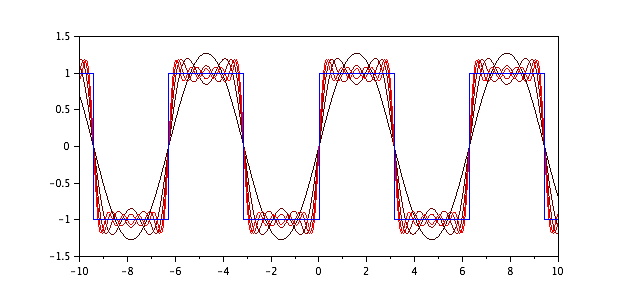
\includegraphics[scale=0.6]{ex1_fig1_1.png}\\*
				\caption{\label{ex1_figure1_1}Courbe de la fonction $f$.}
			\end{figure}\\
		
			\item Richesse fréquentielle du signal
			\begin{figure}[h!]
				\centering
				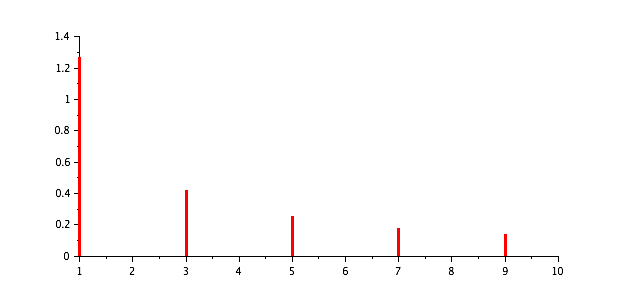
\includegraphics[scale=0.6]{ex1_fig1_2.png}\\*
				\caption{\label{ex1_figure1_2}Richesse du signal $f$.}
			\end{figure}\\
		\end{enumerate}
		\newpage
	
	%2.
		\item $f$ est $2\pi$ périodique, impaire et vaut $f(x)=x, x \in [0,\pi]$ \\ \\
		\begin{enumerate}
			\item Coefficients de Fourier \\ \\
			Les $a(i)$ étant nuls. On obtient ainsi les coefficients suivants pour les $b(i)$ : \\ \\
			\begin{tabular}{l l}
				$b(1) = 2.000000$ & \hspace*{2cm}$b(6) = -0.333333$\\
				$b(2) = -1.000000$ & \hspace*{2cm}$b(7) = 0.285714$\\
				$b(3) = 0.666667$ & \hspace*{2cm}$b(8) = -0.250000$\\
				$b(4) = -0.500000$ & \hspace*{2cm}$b(9) = 0.222222$\\
				$b(5) = 0.400000$ & \hspace*{2cm}$b(10) = -0.200000$\\
			\end{tabular}\\ \\
			\item Série de Fourier \\ \\ \\ \\ \\ \\ \\ \\ \\ \\ \\ \\ \\ \\ \\

			\item Graphe original et ses dix premières approximations
			\begin{figure}[h!]
				\centering
				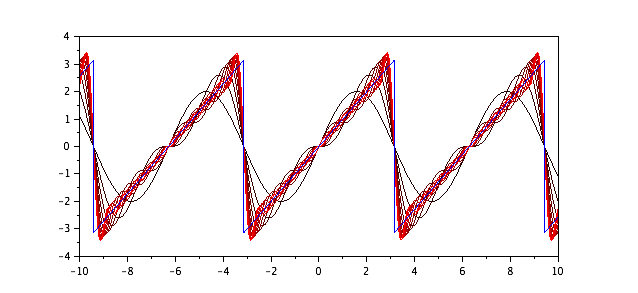
\includegraphics[scale=0.6]{ex1_fig2_1.png}\\*
				\caption{\label{ex1_figure2_1}Courbe de la fonction $f$.}
			\end{figure}\\
		
			\item Richesse fréquentielle du signal
			\begin{figure}[h!]
				\centering
				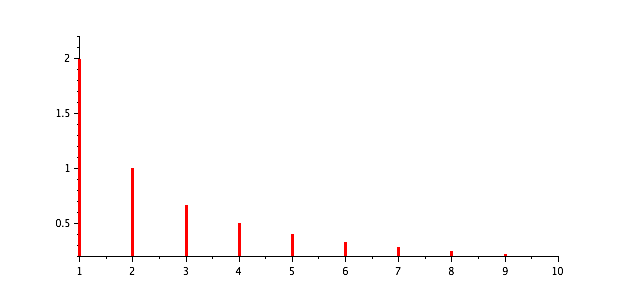
\includegraphics[scale=0.6]{ex1_fig2_2.png}\\*
				\caption{\label{ex1_figure2_2}Richesse du signal $f$.}
			\end{figure}\\
		\end{enumerate}
				\newpage
		
		%3.
		\item $f$ est $2\pi$ périodique, paire et vaut $f(x)=x, x \in [0,\pi]$ \\ \\
		\begin{enumerate}
			\item Coefficients de Fourier \\ \\
			Les $b(i)$ étant nuls. On obtient ainsi les coefficients suivants pour les $a(i)$ : \\ \\
			\begin{tabular}{l l}
				$a(1) = 1.273240$ & \hspace*{2cm}$a(6) = -0.000000$\\
				$a(2) = 0.000000$ & \hspace*{2cm}$a(7) = 0.025984$\\
				$a(3) = 0.141471$ & \hspace*{2cm}$a(8) = 0.000000$\\
				$a(4) = 0.000000$ & \hspace*{2cm}$a(9) = 0.015719$\\
				$a(5) = 0.050930$ & \hspace*{2cm}$a(10) = 0.000000$\\
			\end{tabular}\\
			avec $a(0) = 3.141593$\\ \\
			\item Série de Fourier \\ \\ \\ \\ \\ \\ \\ \\ \\ \\ \\ \\ \\

			\item Graphe original et ses dix premières approximations
			\begin{figure}[h!]
				\centering
				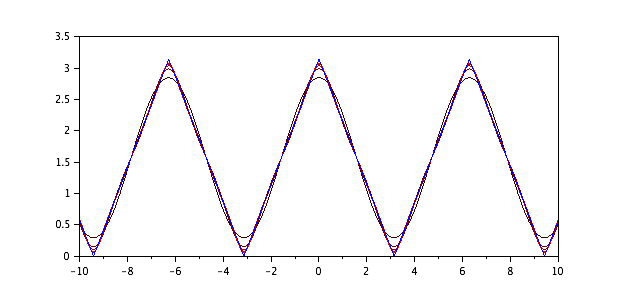
\includegraphics[scale=0.6]{ex1_fig3_1.png}\\*
				\caption{\label{ex1_figure3_1}Courbe de la fonction $f$.}
			\end{figure}\\
		
			\item Richesse fréquentielle du signal
			\begin{figure}[h!]
				\centering
				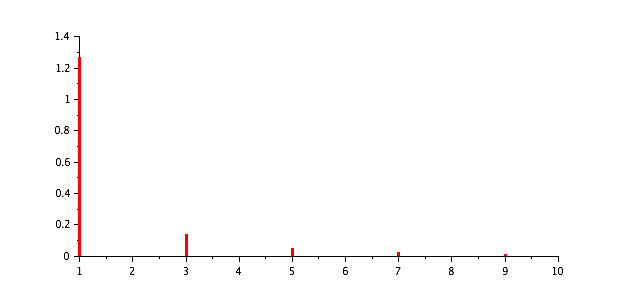
\includegraphics[scale=0.6]{ex1_fig3_2.png}\\*
				\caption{\label{ex1_figure3_2}Richesse du signal $f$.}
			\end{figure}\\
		\end{enumerate}
				\newpage
		
		%4.
		\item $f$ est $2\pi$ périodique, paire et vaut $f(x)=x^{2}, x \in [0,\pi]$ \\ \\
		\begin{enumerate}
			\item Coefficients de Fourier \\ \\
			Les $b(i)$ étant nuls. On obtient ainsi les coefficients suivants pour les $a(i)$ : \\ \\
			\begin{tabular}{l l}
				$a(1) = -4.000000$ & \hspace*{2cm}$a(6) = 0.111111$\\
				$a(2) = 1.000000$ & \hspace*{2cm}$a(7) = -0.081633$\\
				$a(3) = -0.444444$ & \hspace*{2cm}$a(8) = 0.062500$\\
				$a(4) = 0.250000$ & \hspace*{2cm}$a(9) = -0.049383$\\
				$a(5) = -0.160000$ & \hspace*{2cm}$a(10) = 0.040000$\\
			\end{tabular}\\
			avec $a(0) = 6.579736$\\ \\
			\item Série de Fourier \\ \\ \\ \\ \\ \\ \\ \\ \\ \\ \\ \\ \\

			\item Graphe original et ses dix premières approximations
			\begin{figure}[h!]
				\centering
				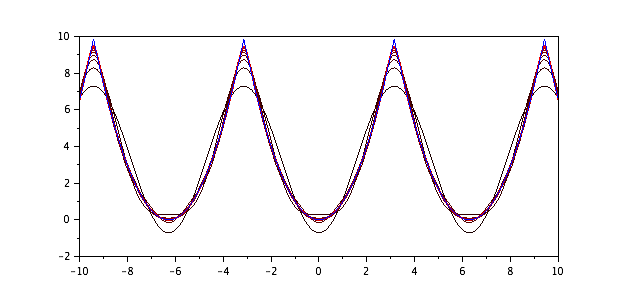
\includegraphics[scale=0.6]{ex1_fig4_1.png}\\*
				\caption{\label{ex1_figure4_1}Courbe de la fonction $f$.}
			\end{figure}\\
		
			\item Richesse fréquentielle du signal
			\begin{figure}[h!]
				\centering
				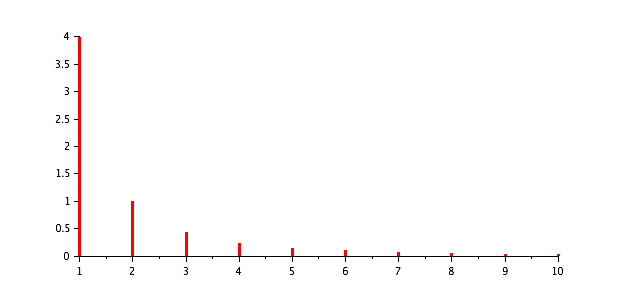
\includegraphics[scale=0.6]{ex1_fig4_2.png}\\*
				\caption{\label{ex1_figure4_2}Richesse du signal $f$.}
			\end{figure}\\
		\end{enumerate}
		\newpage
		
		%5.
		\item $f$ est $2\pi$ périodique, impaire et vaut $f(x)=x(\pi + |x|), x \in [-\pi,\pi]$ \\ \\
		\begin{enumerate}
			\item Coefficients de Fourier \\ \\
			Les $a(i)$ étant nuls. On obtient ainsi les coefficients suivants pour les $b(i)$ : \\ \\
			\begin{tabular}{l l}
				$b(1) = 2.546479$ & \hspace*{2cm}$b(6) = 0.000000$\\
				$b(2) = 0.000000$ & \hspace*{2cm}$b(7) = 0.007424$\\
				$b(3) = 0.094314$ & \hspace*{2cm}$b(8) = -0.000000$\\
				$b(4) = -0.000000$ & \hspace*{2cm}$b(9) = 0.003493$\\
				$b(5) = 0.020372$ & \hspace*{2cm}$b(10) = -0.000000$\\
			\end{tabular}\\ \\
			\item Série de Fourier \\ \\ \\ \\ \\ \\ \\ \\ \\ \\ \\ \\ \\ \\

			\item Graphe original et ses dix premières approximations
			\begin{figure}[h!]
				\centering
				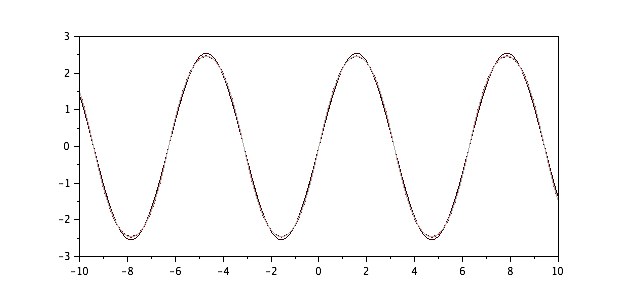
\includegraphics[scale=0.6]{ex1_fig5_1.png}\\*
				\caption{\label{ex1_figure5_1}Courbe de la fonction $f$.}
			\end{figure}\\
		
			\item Richesse fréquentielle du signal
			\begin{figure}[h!]
				\centering
				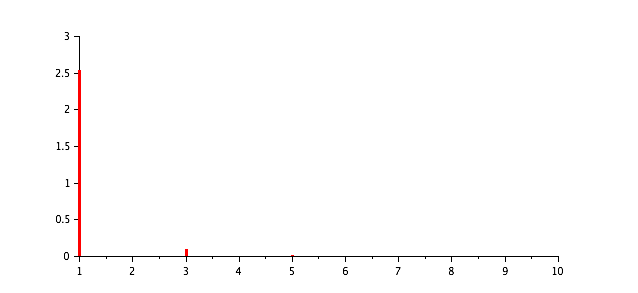
\includegraphics[scale=0.6]{ex1_fig5_2.png}\\*
				\caption{\label{ex1_figure5_2}Richesse du signal $f$.}
			\end{figure}\\
		\end{enumerate}

		
	\end{enumerate}
\newpage



	

%Exercice 2
\chapter{Etude de fonctions}
% 1
	\begin{enumerate}
	\item \[f(x)=(sin\,x)^{1/3}\]
	La fonction f est définie sur l'intervalle ($-\pi;\pi$). Elle est compos\'ee d'une fonction sinus, ce qui la rend impaire. Elle n'admet aucune valeur interdite et on a $f(0^+)=f(0^-)=\sqrt{0}=0$. Elle est donc continue.
	\begin{figure}[h!]
		\centering
		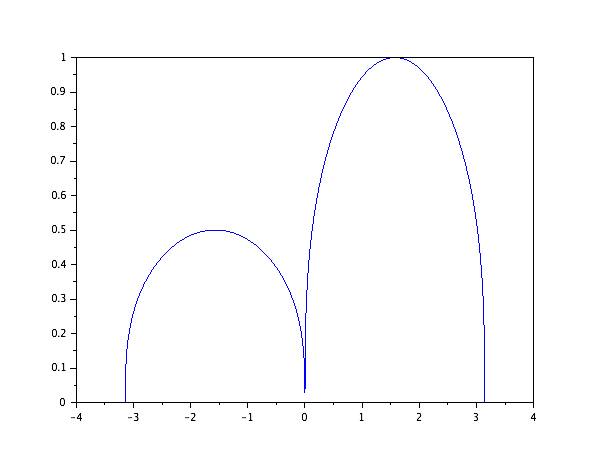
\includegraphics[scale=0.6]{ex2_fig1.png}
		\caption{\label{figure1}Courbe de la fonction $f$.}
		\end{figure}
		\\
	Sa d\'eriv\'ee est \[f'(x)=\frac{1}{3} cos x (sin\,x)^{-2/3}\] Elle admet une asymptote verticale en $0$ et n'est donc pas continue.
	La fonction $f$ est continue mais non d\'erivable sur ($-\pi;\pi$).
	% Faut-il ajouter le programme Scilab ? Que veux dire "Commenter" ?
	\newpage
% 2
	\item \[f(x)=(sin\,x)^{4/3}\]
	La fonction f est définie sur l'intervalle ($-\pi;\pi$). Elle n'admet aucune valeur interdite et on a $f(0^+)=f(0^-)=\sqrt[3]{0}=0$. Elle est donc continue.
	\begin{figure}[h!]
		\centering
		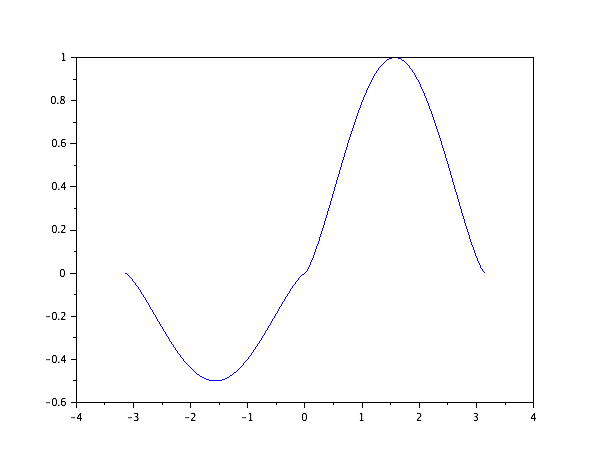
\includegraphics[scale=0.6]{ex2_fig2.png}
		\caption{\label{figure2}Courbe de la fonction $f$.}
		\end{figure}
		\\
	Sa d\'eriv\'ee est \[f'(x)=\frac{4}{3} cos\,x (sin\,x)^{1/3}\] Elle n'admet pas d'asymptote et est donc continue.
	La fonction $f$ est continue et d\'erivable, donc r\'eguli\`ere.
	\newpage
% 3
	\item \[f(x)=
  \left\{
      \begin{aligned}
        cos\,x\quad , si\quad x > 0\\
        -cos\,x\quad ,si\quad x \le 0\\
      \end{aligned}
    \right.\]
	La fonction f est définie sur l'intervalle ($-\pi;\pi$). Elle n'admet aucune valeur interdite et on a $f(0^+)=1$ et $f(0^-)=-1$. Elle n'est donc pas continue en 0.
	\begin{figure}[h!]
		\centering
		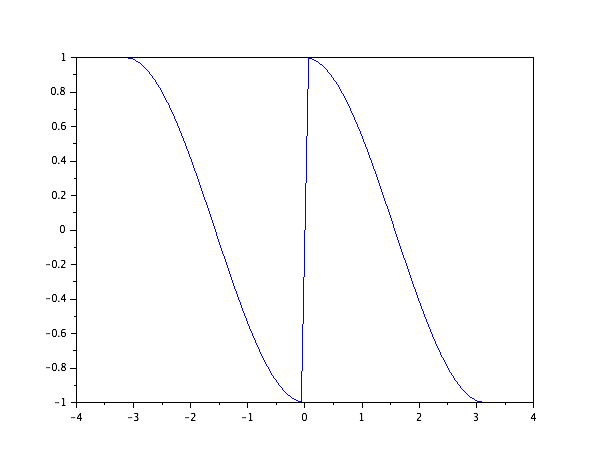
\includegraphics[scale=0.6]{ex2_fig3.png}
		\caption{\label{figure3}Courbe de la fonction $f$.}
		\end{figure}
		\\
	Elle est d\'erivable par morceaux et sa d\'eriv\'ee est \[f'(x)=
  \left\{
      \begin{aligned}
        -sin\,x\quad , si\quad x > 0\\
        sin\,x\quad ,si\quad x \le 0\\
      \end{aligned}
    \right.\] \\
	La fonction $f$ est continue par morceaux et d\'erivable par morceaux, donc r\'eguli\`ere par morceaux.
	\newpage
% 4
	\item \[f(x)=
  \left\{
      \begin{aligned}
        sin\,x\quad , si\quad x > 0\\
        -sin\,2x\quad ,si\quad x \le 0\\
      \end{aligned}
    \right.\]
	La fonction f est définie sur l'intervalle ($-\pi;\pi$). Elle n'admet aucune valeur interdite et on a $f(0^+)=f(0^-)=0$. Elle est donc continue.
	\begin{figure}[h!]
		\centering
		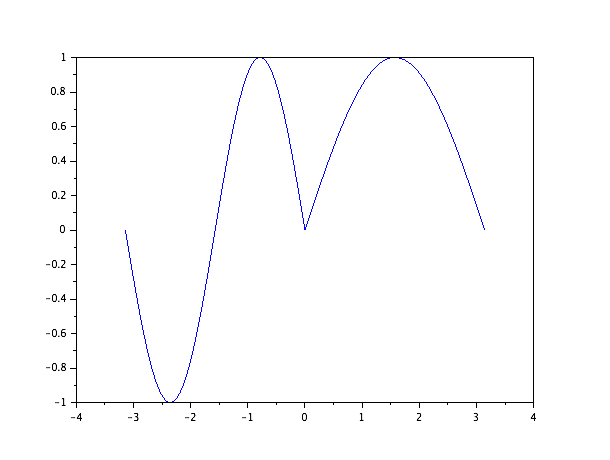
\includegraphics[scale=0.6]{ex2_fig4.png}
		\caption{\label{figure4}Courbe de la fonction $f$.}
		\end{figure}
		\\
	Elle est d\'erivable par morceaux et sa d\'eriv\'ee est \[f'(x)=
  \left\{
      \begin{aligned}
        cos\,x\quad , si\quad x > 0\\
        -2cos\,2x\quad ,si\quad x \le 0\\
      \end{aligned}
    \right.\]
	La fonction $f$ est continue et d\'erivable par morceaux, donc r\'eguli\`ere par morceaux.
	\newpage
% 5
	\item \[f(x)=
  \left\{
      \begin{aligned}
        (sin\,x)^{1/5}\quad , si\quad x < \pi/2\\
        -cos\,x\quad ,si\quad x \ge \pi/2\\
      \end{aligned}
    \right.\]
	La fonction f est définie sur l'intervalle ($-\pi;\pi$). Elle n'admet aucune valeur interdite et on a $f(0^+)=f(0^-)=\sqrt{0}=0$ et $f(\pi/2)=0$ et $\lim\limits_{\substack{x \rightarrow \pi/2 \\ x>\pi/2}} f(x)$. Elle est continue en 0 mais pas en $\pi/2$, elle est donc continue par morceaux.
	\begin{figure}[h!]
		\centering
		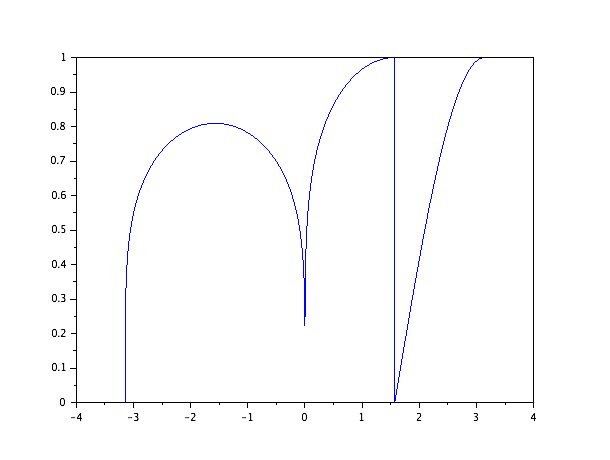
\includegraphics[scale=0.6]{ex2_fig5.png}
		\caption{\label{figure5}Courbe de la fonction $f$.}
		\end{figure}
		\\
	Elle est d\'erivable par morceaux et sa d\'eriv\'ee est \[f'(x)=
  \left\{
      \begin{aligned}
        \frac{1}{5}cos\,x\,(sin\,x)^{1/5}\quad , si\quad x < \pi/2\\
        sin\,x\quad ,si\quad x \ge \pi/2\\
      \end{aligned}
    \right.\]
	La fonction $f$ est continue par morceaux et dérivable par morceaux, donc régulière par morceaux.
	\end{enumerate}
%Exercice 3
\chapter{Phénomène de Gibbs}
\section{Démonstration}
Soit f la fonction 2$\pi$-périodique et impaire telle que $f(x) = 1$ sur $[0; \pi]$.\\

Nous allons montrer que \[S_{f(x)}=\frac{4}{\pi}\sum\limits_{n=0}^{\infty}\frac{sin(2k-1)}{2k-1}\]

Nous savons que $S_{f(x)}=\displaystyle\sum\limits_{n=0}^{\infty} b_{n}sinnx$, car f est impaire.\\
Or, \begin{eqnarray*}
b_{n}&=&\frac{1}{\pi}\int_{-\pi}^{\pi}f(x)sinnx\\
		 &=&\frac{1}{\pi}\int_{-\pi}^{0}f(x)sinnx\,+\,\frac{1}{\pi}\int_{0}^{\pi}f(x)sinnx\\
		 &=&-\frac{1}{\pi}\int_{-\pi}^{0}sinnx\,+\,\frac{1}{\pi}\int_{0}^{\pi}sinnx\\
		 &=&\frac{1}{\pi}\int_{0}^{\pi}sinnx\,+\,\frac{1}{\pi}\int_{0}^{\pi}sinnx\\
		 &=&\frac{2}{\pi}\int_{0}^{\pi}sinnx\\
		&=&\frac{2}{\pi}\left[\frac{-cosnx}{k}\right]_0^\pi\\
		 &=&\frac{2}{\pi}\left(-\frac{cosn\pi}{n}+\frac{1}{n}\right)\\
		 &=&\frac{2}{\pi}\left(-\frac{cosn\pi}{n}+\frac{1}{n}\right)\\
	\end{eqnarray*}
D'o\`u \begin{eqnarray*}
S_{f(x)}&=&\frac{2}{\pi}\displaystyle\sum\limits_{n=0}^{\infty}\frac{1-cosnx}{n}sinnx\\
		&=&\frac{2}{\pi}\displaystyle\sum\limits_{n=0}^{\infty}\frac{1-(-1)^{n}}{n}sinnx\\
		&=&\frac{2}{\pi}\sum\limits_{n\,pair}^{\infty}\frac{1-(-1)^{n}}{n}sinnx\,+\,\frac{2}{\pi}\sum\limits_{n\,impair}^{\infty}\frac{1-(-1)^{n}}{n}sinnx\\
		&=&\frac{4}{\pi}\sum\limits_{n\,impair}^{\infty}\frac{sinnx}{n}\\
		&=&\frac{4}{\pi}\sum\limits_{n=1}^{\infty}\frac{sin(2k-1)x}{2k-1}\qquad,\;\text{o\`u}\;n=2k-1\;,\;k\,\in\,\pmb{\mathbb{R}}\\
	\end{eqnarray*}
\section{Approximations de Fourier}

\section{Explication du ph\'enom\`ene}

%Exercice 4
\chapter{Application des série de Fourier}
\section{La corde pincée}
\section{La corde frappée}

%Exercice 5
\chapter{Equation de la chaleur}

%Complément au TP
\chapter{Compléments}
\section{Finance}
\section{Informatique}

%Test de texte
Comme le disait Jean de la Fontaine dans sa fable :
\begin{quote}
Rien de sert de courir, il faut partir à point.
\end{quote}


\end{document}